\documentclass{beamer}

\usepackage{amsmath, amssymb, hyperref, graphics, wasysym}
\usepackage{tikz}
\usepackage{mathpazo}
\usetikzlibrary{cd}

\newcommand{\C}{\mathbb{C}}
\newcommand{\Z}{\mathbb{Z}}
\newcommand{\R}{\mathbb{R}}

\title{MAS439 Lecture 7 \\ Isomorphism Theorem}

\date{October 13th}

\begin{document}

\begin{frame}
\titlepage
\end{frame}


\begin{frame}{}
Last week we motivated and defined the quotient ring $R/I$, proved it was a ring, and looked at some examples.

Today is centred around the first isomorphism theorem, which states that for any homomorphsim $\varphi:R\to S, \textrm{Im}(\varphi)\cong R/\ker(\varphi)$.  However, the possibly new to you part, and a main player, is the Universal Property of quotient rings.

\end{frame}

\begin{frame}[fragile]{The Universal Property for Quotient rings}
Suppose that $\varphi:R \to S$ is a ring homomorphism such that $I\subset \ker(\varphi)$, and let $p:R\to R/I$ be the quotient map.   Then there exists a unique ring homomorphism $\overline{\varphi}:R/I\to S$ satisfying $\varphi=\overline{\varphi}\circ p$.

\begin{block}{Put another way}
The following diagram commutes:
\begin{center}
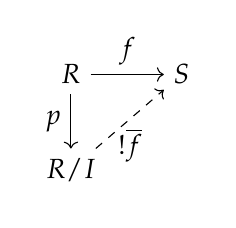
\begin{tikzpicture}[every node/.style={midway}]
\matrix[column sep={4em,between origins},
        row sep={2em}] at (0,0)
{ \node(R)   {$R$}  ;  & \node(S) {$S$}; \\
  \node(R/I) {$R/I$  };                   \\};
\draw[<-] (R/I) -- (R) node[anchor=east]  {$p$};
\draw[->, dashed] (R/I) -- (S) node[anchor=north]  {$ !\overline{f}$};
\draw[->] (R)   -- (S) node[anchor=south] {$f$};
\end{tikzpicture}
\end{center}
\end{block}

\end{frame}

\begin{frame}{What the universal property ``really means''}
\begin{block}{Universal property as a slogan:}
Maps out of $R/I$ are the same thing as maps out of $R$ whose kernel contains $I$
\end{block}

This property \emph{defines} the quotient ring $R/I$.

\begin{block}{Categorical thinking as a slogan:}
Understand an object by understanding how it relates to other objects.  As an example, if you know all the maps out of an object, you know the object.
\end{block}
\end{frame}


\begin{frame}{Proof of the Universal Property}

\begin{block}{Uniqueness of $\overline{\varphi}$:}
If $[r]\in R/I$, we want to know $\overline{\varphi}([r])$.  Noting that $[r]=p(r)$, we see that having $\varphi=\overline{\varphi}\circ p$ is equivalent to: 

$$\overline{\varphi}([r])=\overline{\varphi}(p(r))=\varphi(r)$$
\end{block}

Thus, we take as a definition $\overline{\varphi}([r]):=\varphi(r)$ to guarantee $\varphi=\overline{\varphi}\circ p$. 

\begin{block}{What's left?} 
\begin{itemize}
\item Show $\overline{\varphi}$ is a homomorphism; 
\item We are defining what $\overline{\varphi}$ in terms of representatives, so we must show it's well defined.
\end{itemize}
\end{block}
\end{frame}

\begin{frame}{Proof of the Universal Property}

\begin{block}{$\overline{\varphi}$ is a ring homomorphism:}

 We check addition:
\begin{align*}
\overline{\varphi}([s]+[r]) & =\overline{\varphi}([r+s]) \\
&=\varphi(r+s) \\
& =\varphi(r)+\varphi(s) \\
&=\overline{\varphi}([r])+\overline{\varphi}([s])
\end{align*}

Multiplication and unit are similar.
\end{block}
\end{frame}

\begin{frame}{Proof of the Universal Property}
\begin{block}{ $\overline{\varphi}$ is well defined:}

  Suppose that $r\sim s$; we must show $\overline{\varphi}([s])=\overline{\varphi}([r])$, i.e., that $\varphi(r)=\varphi(s)$.


But $r\sim s$ means $r=s+i$ for $i\in I$, so 
$$\varphi(r)=\varphi(s+i)=\varphi(s)+\varphi(i)=\varphi(s)$$
since $I\subset \ker(\varphi)$.

\end{block}
\end{frame}


\begin{frame}{Digging old tools out of the shed}

To prove the isomorphism theorem, we are going to use the following two facts we've already seen:

\begin{itemize}
\item Any ring homomorphism $\varphi:R\to S$ factors as the surjection from $\varphi:R \to \textrm{Im}(\varphi)$ and the inclusion $i:\textrm{Im}(\varphi)\to S$

\item A homomorphism $\varphi$ is injective if and only if $\ker(\varphi)=0$.

\end{itemize}



\end{frame}

\begin{frame}[fragile]{Isomorphism Theorem Restated}

Any ring homomorphism $\varphi:R\to S$ can be written uniquely in the form 
$$\varphi=i\circ\overline{\varphi}^\prime\circ p$$
 where
\begin{itemize}
\item $p:R\to R/\ker{\varphi}$ is the quotient map
\item $\overline{\varphi}^\prime:R/\ker(\varphi)\to \textrm{Im}(\varphi)$ is an isomorphism
\item $i:\textrm{Im}(\varphi)\to S$ is the inclusion
\end{itemize}
\begin{center}
\begin{tikzcd}
R  \arrow[r, "\varphi"] \arrow[d, "p"] & S \arrow[<-, d, "i"] \\
R/\ker{\varphi} \arrow[r, "\overline{\varphi}^\prime"] & \textrm{Im}(\varphi) 
\end{tikzcd}
\end{center}

\end{frame}


\begin{frame}[fragile]{Proof of the First isomorphism theorem}

From the toolshed, we have a surjective map $\tilde{\varphi}:R\to\textrm{Im}(\varphi)$ with $\varphi=i\circ\tilde{\varphi}$.  That is, we have the upper right triangle commutes:
\begin{center}
\begin{tikzcd}
R  \arrow[r, "\varphi"] \arrow[d, "p"]\arrow[rd, "\tilde{\varphi}"] & S \arrow[<-, d, "i"] \\
R/\ker{\varphi} \arrow[r, "\overline{\varphi}^\prime"] & \textrm{Im}(\varphi) 
\end{tikzcd}
\end{center}

Furthermore, since $i$ is injective, we have $\ker{\tilde{\varphi}}=\ker{i\circ\varphi}=\ker{\varphi}$

\end{frame}

\begin{frame}[fragile]{Proof of the first isomorphism theorem}
\begin{center}
\begin{tikzcd}
R  \arrow[r, "\varphi"] \arrow[d, "p"]\arrow[rd, "\tilde{\varphi}"] & S \arrow[<-, d, "i"] \\
R/\ker{\varphi} \arrow[r, "\overline{\varphi}^\prime"] & \textrm{Im}(\varphi) 
\end{tikzcd}
\end{center}
To get the bottom triangle, we apply the universal property of $R/\ker{\varphi}$ to $\tilde{\varphi}$ to construct the map $\overline{\varphi}^\prime$.

\begin{itemize}
\item Bottom triangle commutes by universal property
\item $\overline{\varphi}^\prime$ surjective since $\tilde{\varphi}$ is
\item $\overline{\varphi}^\prime$ injective since:
 

$$\overline{\varphi}^\prime([r])=0\iff \tilde{\varphi}(r)=0\iff r\in \ker(\tilde{\varphi})\iff r\sim 0_R$$

\end{itemize}


\end{frame}


\begin{frame}[plain,c]

\begin{center}

\Huge

\usebeamercolor[fg]{frametitle}
$\twonotes$ Let's all go to the lobby $\twonotes$ \\ $\twonotes$ Let's all go to the lobby $\twonotes$ \\
(2 minute intermission)
\end{center}

\end{frame}

\begin{frame}{Application of Isomorphism theorem: $\R[x]/(x^2+1)\cong\C$}

Evaluation at $i$ gives a map 
$$f:\R[x]\to \C\quad \quad f:p\mapsto p(i)$$
\begin{itemize}
\item We have $x^2+1\in\ker(f)$, and so by definition $(x^2+1)\in\ker(f)$
\item By universal property, get a map $\overline{f}:R[x]/(x^2+1)\to\C$
\item First isomorphism theorem says this map is an $\cong$ if $\ker(f)=(x^2+1)$
\item If $g\notin (x^2+1)$, can see $g\notin \ker(f)$ using division algorithm:

$$g=(x^2+1)p(x)+ax+b\quad \implies\quad f(g)=ai+b $$


\end{itemize}


\end{frame}

\begin{frame}{The pullback of an ideal is an ideal}


\begin{lemma}
Let $f:R\to S$ a map, $I\subset S$ an ideal.  Then $f^{-1}(I)\subset R$ an ideal
\end{lemma}


\begin{proof}
Suppose $a,b\in f^{-1}(I), r\in R$
\begin{itemize}
\item $f^{-1}(I)$ is nonempty since it contains 0.
\item We have $a+b\in f^{-1}(I)$ since
$$f(a+b)=f(a)+f(b)\in I$$
\item We have $r\cdot a\in f^{-1}(I)$ since
$$f(ar)=f(a)f(r)\in I$$
\end{itemize}
\end{proof}


\end{frame}

\begin{frame}
\begin{lemma} If $I\subset J\subset R$ are two ideals, then 

$$J/I=\left\{[r]\in R/I : r\in J\right\}$$
is an ideal in $R/I$.
\end{lemma}

\begin{proof}
Need to check:
\begin{itemize}
\item Well defined: i.e., if $[r_1]=[r_2]$ then $[r_1]\in J/I\iff [r_2]\in J/I$. 
\item nonempty
\item Closed under addition
\item closed under multiplication by elements of $R/I$.
\end{itemize}
\end{proof}
\end{frame}

\begin{frame}
The lemmas give us maps back and forth between ideals of $R$ containing $I$ and ideals of $R/I$:

\begin{itemize}
\item If $K\subset R/I$ an ideal, then $I\subset p^{-1}(K)\subset R$ an ideal.
\item If $I\subset J\subset K$, then $J/I$ an ideal of $R/i$.
\end{itemize}

\begin{lemma}The above maps are inverse

\end{lemma}
The fact that $p^{-1}(J/I)=J$ is exactly the definition.

Now suppose $K\subset R/I$ an ideal; we must show $p^{-1}(K)/I=K$.
\begin{itemize}
\item If $[a]\in p^{-1}(K)$, then $a\in p^{-1}(K)$, so $p(a)=[a]\in K$.
\item If $[a]\in K$, then $a\in p^{-1}(K)$, and so $[a]\in p^{-1}(K)/I$
\end{itemize}
\end{frame}

\begin{frame}{A corollary}

\begin{lemma} If $R$ is a principal ideal domain, then $R/I$ is a principal ideal domain.
\end{lemma}

\begin{proof}
Suppose that $K\susbet R/I$ is an ideal.  Then $K$ is of the form $J/I$ for some ideal $I\subset J\subset R$.  Since $R$ is a principal ideal domain, $J=(r)$.  But then $\big([r]\big)$ generates $J/I$.
\end{proof}

Since $\mathbb{Z}$ is a principal ideal domain, we have $\mathbb{Z}/k$ is.


\end{frame}




\begin{frame}{Third isomorphism theorem}
\begin{theorem}
If $I\subset J\subset R$ ideals, then $R/J\cong (R/I)\cong (J/I)$
\end{theorem}

\begin{proof}
We construct a map $f:R/J\to R/I$ by taking $f([r]_{R/J})=[r]_{R/I}$.
Need to check:
\begin{itemize}
\item Well defined
\item Surjective
\item ring homomorphism
\item $\ker(f)=J/I$
\end{itemize}

Then it follows from first isomorphism theorem.

\end{proof}

\end{frame}


\begin{frame}{Examples}

\begin{itemize}
\item What do we get from $(2)\subset (8)\subset \mathbb{Z}$? 

$$(\Z/8)/(2)\cong\Z/2$$
\item What do we get from $(2)\subset (2,x^2+x+1)\subset \Z[x]$?
\begin{align*}
\Z[x]/(2,x^2+x+1)& \cong \big(\Z[x]/(2)\big)/(2,x^2+x+1)\\
& \cong \mathbb{F}_2[x]/(x^2+x+1) \\
& \cong \mathbb{F}_4
\end{align*}
\end{itemize}
\end{frame}


\end{document}
